%!TEX root = ./report.tex
\section{Solution}
The final product combines several technologies to attain an extendable solution with two reusable Xtend workflows at its core. The setup allows the user to edit a subset of IFC in a generated Eclipse editor in between the two workflows. The main model is stored on a BIMServer for merging, versioning and extensibility purposes, as this section will further explain.

\subsection{Server Side}
As described in (TODO reference Kan Jørgensens workflow document) a construction model and a plumbing model are combined into one single model that needs to be verified for consistency. So called openings, i.e. holes, in walls and floors need to be in place where the plumbing model describes flow segments to be installed. We let a BIMServer handle this merging of models. Many tools exist for this job, but the special advantage of the BIMServer is that it also provides version control, a java client library as well as conversion tools enabling the user to extract the saved building in other formats.

\subsection{Client Side}
Figure \ref{fig:IFC2PipesWorkflow} shows the IFC to Pipes workflow retrieving an IFC model from the BIMServer as XML, processing it to the corresponding ecore instance, extracting the pipes and opening elements and converting these to an editable DSL instance saved to disk as an XMI file. The XML file loaded from the server is saved to the local disk for use by the second workflow explained below.

\begin{figure}[htbp]
    \centering
        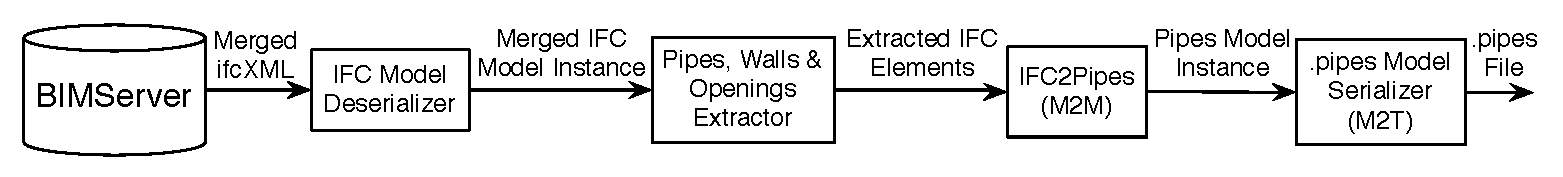
\includegraphics[width=120mm]{images/IFC2Pipes.pdf}
    \caption{IFC to Pipes DSL workflow}
    \label{fig:IFC2PipesWorkflow}
\end{figure}

The second workflow is depicted on Figure \ref{fig:Pipes2IFCWorkflow}, where the edited XMI file is loaded into a Main model updater workflow module together with a non-updated extracted instance of the main model. Notice how the extraction is loaded in using the same workflow modules as in the first workflow, except the XML file is not fetched from the server but from the local disk. This makes for an easier update process in the Main Model Updater as the extracted instance is guaranteed to not have changed while the user was editing the XMI file. After the main model instance has been updated to reflect the users changes it is converted to XML and this new file is saved back to the BIMServer.

\begin{figure}[htbp]
    \centering
        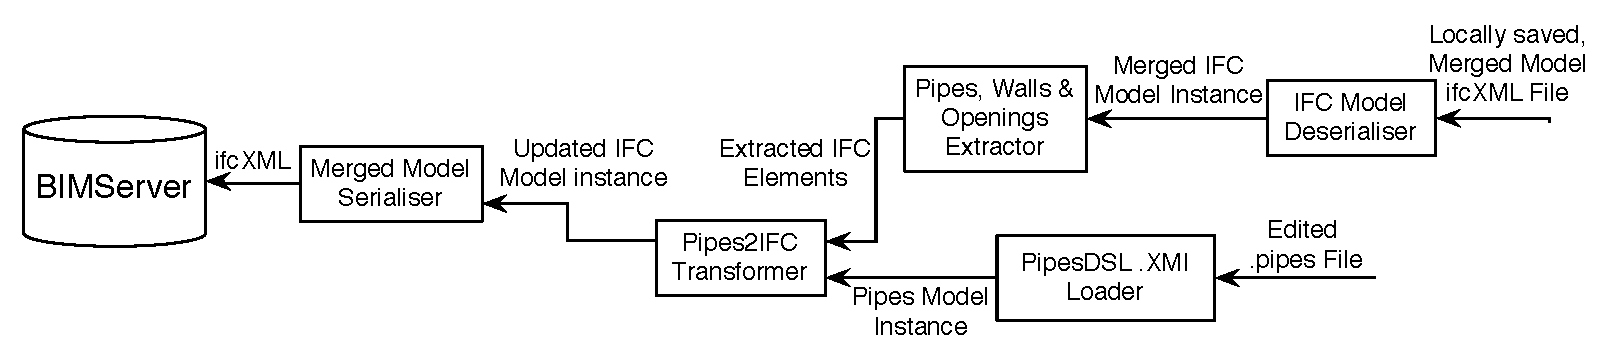
\includegraphics[width=120mm]{images/Pipes2IFC.pdf}
    \caption{Pipes DSL to IFC workflow}
    \label{fig:Pipes2IFCWorkflow}
\end{figure}






